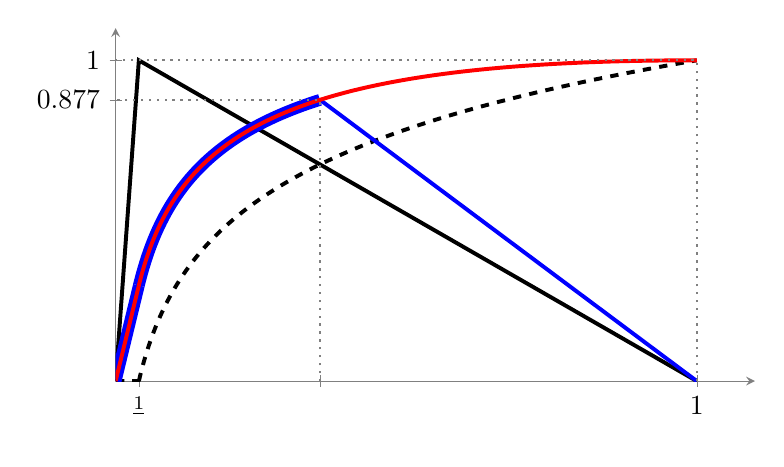
\begin{tikzpicture}[scale=1, transform shape]
\begin{axis}[
axis line style=gray,
axis lines=middle,
xlabel = $\quant$,
xtick={0, 0.04, 0.35168, 1},
ytick={0, 0.8767514, 1},
xticklabels={0, $\frac{1}{\constantH}$, $\fquant$, 1},
yticklabels={0, $0.877$, $1$},
xmin=0,xmax=1.1,ymin=-0.0,ymax=1.1,
width=0.8\textwidth,
height=0.5\textwidth,
samples=500]

\addplot[black!100!white, line width=0.5mm] (0, 0) -- (0.04, 1) -- (1, 0);

\addplot[domain=0:0.04, dashed, line width=0.5mm] (x, {0});
% \addplot[domain=0.04:1, red, line width=0.5mm] (x, {(1 + 25 / 24 * (ln(x) + ln(25) - x + 0.04) - 25 / 24 * (1 - x) / 3.3529956509});
\addplot[domain=0.04:1, dashed, line width=0.5mm] (x, {(1 + 25 / 24 * (ln(x) + ln(25) - x + 0.04) - 25 / 24 * (1 - x)) / 3.3529956509});


\addplot[blue, line width=1.5mm] (0, 0) -- (0.04, 0.2982407);
\addplot[domain=0.04:0.35168, blue, line width=1.5mm] (x, {(1 + 25 / 24 * (ln(x) + ln(25) - x + 0.04)) / 3.3529956509});
\addplot[blue, line width=0.5mm] (0.35168, 0.8767514) -- (1, 0);

\addplot[red, line width=0.5mm] (0, 0) -- (0.04, 0.2982407);
\addplot[domain=0.04:1, red, line width=0.5mm] (x, {(1 + 25 / 24 * (ln(x) + ln(25) - x + 0.04)) / 3.3529956509});



\addplot[dotted, gray, line width=0.3mm] (0.35168, 0) -- (0.35168, 0.8767514) -- (0, 0.8767514);

\addplot[dotted, gray, line width=0.3mm] (1, 0) -- (1, 1) -- (0, 1);



\end{axis}

\end{tikzpicture}